\chapter{Multiple-View Geometry}
\label{ch:multiview}

\begin{objectives}
\begin{itemize}
  \item Derive the epipolar constraint, the essential and fundamental matrices, epipoles and epipolar lines.
  \item Recover relative motion from correspondences: the eight-point algorithm with normalization, the five-point and two-point methods, and the
        decomposition of the essential matrix.
  \item Understand homographies between views, the pure-rotation case, and the degeneracies of relative-pose estimation.
  \item Use RANSAC to reject outliers, size its iteration count, and set thresholds in the right units.
  \item Triangulate points by midpoint, linear and Gauss--Newton methods, and quantify triangulation accuracy.
  \item Understand bundle adjustment, its sparsity and its gauge freedom: the batch problem the MSCKF approximates.
\end{itemize}
\end{objectives}

% ==============================================================================
\section{Epipolar geometry}

\subsection{The epipolar constraint}

Two cameras observe the same 3D point. Let the coordinates of the point in the two camera frames be $X_1$ and $X_2$, related by the rigid motion
\begin{equation}
  X_2 = R\,X_1 + t, \qquad R = R_{c_2c_1},\quad t = p_{c_2c_1},
\end{equation}
and let $\bar x_1 = X_1/Z_1$ and $\bar x_2 = X_2/Z_2$ be the bearings (homogeneous normalized coordinates).

\begin{theorem}[Epipolar constraint]
\label{thm:epipolar}
\index{epipolar constraint}\index{essential matrix}
Every correspondence of a rigid point satisfies
\begin{equation}
  \bar x_2\T\,E\,\bar x_1 = 0, \qquad E = \sx{t}\,R .
  \label{eq:epipolar}
\end{equation}
\end{theorem}
\begin{proof}
Cross both sides of $X_2 = RX_1 + t$ with $t$: $\sx{t}X_2 = \sx{t}RX_1$. The left side is orthogonal to $X_2$, so $X_2\T\sx{t}RX_1 = 0$. Dividing by $Z_1Z_2 > 0$ gives
\eqref{eq:epipolar}.
\end{proof}

Geometrically, the two camera centers and the 3D point span a plane, the \emph{epipolar plane}, and the constraint states that the two viewing rays and the baseline
are coplanar (\cref{fig:epipolar}). The constraint involves no depth: it is a statement about bearings only, which is why it is the natural tool for checking tracks
before any 3D reconstruction exists.

\begin{figure}[t]
\centering
\begin{tikzpicture}[scale=1.0]
  \coordinate (C1) at (0,0); \coordinate (C2) at (5,0.3); \coordinate (P) at (2.7,3.4);
  \fill[primarylight, opacity=0.7] (C1) -- (C2) -- (P) -- cycle;
  \draw[thick] (C1) -- (C2) node[midway, below] {baseline $t$};
  \draw[plotgreen, thick] (C1) -- (P); \draw[plotgreen, thick] (C2) -- (P);
  \fill (C1) circle (1.8pt) node[below left] {$C_1$};
  \fill (C2) circle (1.8pt) node[below right] {$C_2$};
  \fill[conv] (P) circle (2pt) node[above] {$p_f$};
  \draw[primary, thick] (0.3,1.5) -- (1.6,1.2) -- (1.6,0.2) -- (0.3,0.5) -- cycle;
  \draw[primary, thick] (3.5,1.3) -- (4.8,1.7) -- (4.8,0.7) -- (3.5,0.3) -- cycle;
  \fill[plotgreen] ($(C1)!0.3!(P)$) circle (1.5pt) node[left, font=\footnotesize] {$\bar x_1$};
  \fill[plotgreen] ($(C2)!0.3!(P)$) circle (1.5pt) node[right, font=\footnotesize] {$\bar x_2$};
  \draw[conv, dashed] (3.6,0.65) -- (4.75,1.45);
  \node[conv, font=\footnotesize, anchor=west] at (5.0,1.25) {epipolar line $E\bar x_1$};
  \node[font=\footnotesize, primary] at (2.6,1.7) {epipolar plane};
\end{tikzpicture}
\caption{Epipolar geometry. The camera centers, the point and both viewing rays lie in one plane. The image of the point in the second camera must therefore lie on
the line where that plane cuts the second image.}
\label{fig:epipolar}
\end{figure}

\subsection{Epipolar lines and epipoles}

Given $\bar x_1$, the vector $\ell_2 = E\bar x_1$ represents a line in the second image (\cref{sec:homogeneous}), the \term{epipolar line}: the corresponding point must lie on
it. Searching for a match can be restricted to this line. All epipolar lines in the second image pass through the \term{epipole} $e_2$, the image of the first camera
center, which satisfies $e_2\T E = 0$ (it is proportional to $t$); symmetrically $Ee_1 = 0$ with $e_1 \propto R\T t$. When the camera moves forward, the epipole is the
\emph{focus of expansion} from which image points flow outward.

\begin{proposition}[Properties of the essential matrix]
\label{prop:essential}
For $t \ne 0$, $E = \sx{t}R$ has rank two and two equal non-zero singular values, $(\|t\|, \|t\|, 0)$. It has five degrees of freedom: three for the rotation and two for the
direction of $t$. Its overall scale, like the scale of $t$, is unobservable.
\end{proposition}
\begin{proof}
$EE\T = \sx{t}RR\T\sx{t}\T = -\sx{t}^2 = \|t\|^2I - tt\T$ by \eqref{eq:skew-sq}, whose eigenvalues are $\|t\|^2$ (twice, on the plane orthogonal to $t$) and $0$ (along $t$). The
singular values of $E$ are their square roots.
\end{proof}

In pixel coordinates, with $\tilde u_i = K\bar x_i$, the constraint reads $\tilde u_2\T F\tilde u_1 = 0$ with the \term{fundamental matrix} $F = K\mT EK\inv$ (seven degrees of freedom,
rank two). The project works with undistorted normalized coordinates throughout, so it uses $E$ directly (Milestone 9).

% ==============================================================================
\section{Estimating relative motion}

\subsection{The eight-point algorithm}

\Cref{eq:epipolar} is linear in the nine entries of $E$. Writing $\bar x_1 = (x_1, y_1, 1)$ and $\bar x_2 = (x_2, y_2, 1)$, each correspondence gives one equation
\begin{equation}
  a\T e = 0, \qquad a = (x_2x_1,\ x_2y_1,\ x_2,\ y_2x_1,\ y_2y_1,\ y_2,\ x_1,\ y_1,\ 1), \qquad e = \vect_{\text{rows}}(E).
\end{equation}
With eight or more correspondences, stack them into $Ae = 0$ and take the unit vector minimizing $\|Ae\|$: the right singular vector of $A$ with the smallest
singular value (\cref{prop:homogeneous-ls}). Noise makes the result an invalid essential matrix, which is projected onto the nearest valid one by replacing its
singular values with $(1, 1, 0)$ (\cref{thm:svd} and Eckart--Young). When the algorithm is applied to pixel coordinates (to estimate $F$), the coordinates must first
be \emph{normalized} (translated to zero mean and scaled to unit average distance from the origin), or the matrix $A$, whose entries range from 1 to $10^5$, is so
badly conditioned that the result is unusable; this is Hartley's normalization.

\subsection{Decomposing the essential matrix}

\begin{proposition}[Motion from the essential matrix]
\label{prop:e-decomposition}
Let $E = U\diag(1, 1, 0)V\T$ with $U, V$ rotations (flip their signs if needed), and $W = \begin{bmatrix}0 & -1 & 0\\ 1 & 0 & 0\\ 0 & 0 & 1\end{bmatrix}$. The rotation and translation
direction are one of the four combinations
\begin{equation}
  R \in \{UWV\T,\ UW\T V\T\}, \qquad t \in \{+u_3,\ -u_3\},
\end{equation}
where $u_3$ is the third column of $U$. Exactly one of the four places triangulated points in front of both cameras.
\end{proposition}

The proof checks that $\sx{u_3}UWV\T$ and $\sx{u_3}UW\T V\T$ both equal $E$ up to sign, and that no other factorizations exist. The four solutions correspond to the second
camera being on either side of the first, facing either forward or backward; the \emph{cheirality} test (positive depth of a triangulated point in both views)
selects the physical one.

\subsection{The five-point and two-point methods}

Five correspondences are the minimum, since $E$ has five degrees of freedom. Nistér's algorithm~\cite{nister2004five} combines the linear constraints of five
correspondences with the cubic constraints that characterize essential matrices ($\det E = 0$ and $2EE\T E - \tr(EE\T)E = 0$) and solves the resulting polynomial system,
returning up to ten candidates. Fewer points per hypothesis means fewer RANSAC iterations, which is why \code{cv::findEssentialMat} uses it.

In VIO the gyroscope supplies the relative rotation $R$ between consecutive frames with high accuracy. With $R$ known, \eqref{eq:epipolar} becomes linear in $t$:
\begin{equation}
  \bar x_2\T\sx{t}R\bar x_1 = t\T\big(R\bar x_1\times\bar x_2\big) = 0 .
\end{equation}
Each correspondence says that $t$ is orthogonal to the vector $c_i = R\bar x_1^{(i)}\times\bar x_2^{(i)}$, so two correspondences determine the direction of $t$ as $c_1\times c_2$. A two-point
hypothesis needs far fewer RANSAC iterations than a five-point one, and it is the outlier-rejection strategy of MSCKF-VIO~\cite{sun2018msckfvio}.

\subsection{Measuring the residual}

The algebraic residual $\bar x_2\T E\bar x_1$ has no geometric meaning. The geometric error of a correspondence is the smallest displacement of $\bar x_1$ and $\bar x_2$ that
makes the constraint hold exactly. Linearizing the constraint in that displacement gives the \emph{Sampson distance}
\begin{equation}
  d_S = \frac{(\bar x_2\T E\bar x_1)^2}{(E\bar x_1)_1^2 + (E\bar x_1)_2^2 + (E\T\bar x_2)_1^2 + (E\T\bar x_2)_2^2},
\end{equation}
the squared residual divided by the squared norm of its gradient with respect to the four image coordinates: the first-order squared distance to the constraint
surface. It is in the units of the coordinates used. With normalized coordinates, a pixel threshold $\tau_{px}$ must be converted to $\tau_{px}/f$ (Milestone 9).

\begin{pitfall}[thresholds in the wrong units]
Calling \code{cv::findEssentialMat} on normalized coordinates with an identity camera matrix and a threshold of ``1.0'' accepts residuals of 1 normalized unit, about
450 pixels: every track becomes an inlier. The threshold must be $\tau_{px}/f$, e.g.\ $1/458 \approx 2.2\times10^{-3}$.
\end{pitfall}

% ==============================================================================
\section{Homographies between views}
\label{sec:homographies}

\paragraph{Planar scenes.} If all points lie on a plane $n\T X_1 = d$ (unit normal $n$ and distance $d$ in the first camera's frame), then $1 = n\T X_1/d$ and
$X_2 = RX_1 + t\,n\T X_1/d$, so
\begin{equation}
  X_2 = \Big(R + \frac{t\,n\T}{d}\Big)X_1, \qquad \bar x_2 \propto H\bar x_1, \quad H = R + \frac{tn\T}{d} .
\end{equation}
\paragraph{Pure rotation.} If $t = 0$, $X_2 = RX_1$ for every point, at any depth: $\bar x_2 \propto R\bar x_1$, the \emph{infinite homography}. In pixels it is $KRK\inv$.

A homography has eight degrees of freedom and is estimated from four or more correspondences by a direct linear transform: each correspondence gives two linear
equations in the nine entries of $H$ (from $\tilde x_2\times H\tilde x_1 = 0$), solved by \cref{prop:homogeneous-ls}.

% ==============================================================================
\section{RANSAC}

Random Sample Consensus~\cite{fischler1981ransac} estimates a model from data containing outliers by hypothesis and verification.

\begin{algorithm}[h]
\caption{RANSAC}
\begin{algorithmic}[1]
\Require data, minimal sample size $s$, threshold $\tau$, confidence $p$
\State best $\gets \emptyset$; $N \gets \infty$; $k \gets 0$
\While{$k < N$}
  \State draw $s$ data points at random; fit candidate models
  \State count inliers with residual $< \tau$; keep the model with the most inliers
  \State update $N$ from the current inlier ratio $w$ with \eqref{eq:ransac-n}; $k \gets k + 1$
\EndWhile
\State refit the model on all inliers of the best hypothesis (least squares)
\end{algorithmic}
\end{algorithm}

If a fraction $w$ of the data are inliers, a random minimal sample is outlier-free with probability $w^s$, and $N$ independent samples all contain an outlier with probability
$(1 - w^s)^N$. Requiring this to be at most $1 - p$ gives the number of iterations
\begin{equation}
  N = \frac{\log(1 - p)}{\log(1 - w^s)} .
  \label{eq:ransac-n}
\end{equation}
\begin{center}\small
\begin{tabular}{@{}l c c c@{}}
\toprule
$p = 0.99$ & $w = 0.9$ & $w = 0.7$ & $w = 0.5$ \\
\midrule
8-point ($s = 8$) & 9 & 78 & 1177 \\
5-point ($s = 5$) & 6 & 26 & 146 \\
2-point ($s = 2$) & 3 & 7 & 17 \\
\bottomrule
\end{tabular}
\end{center}
The exponential dependence on $s$ is why minimal solvers matter, and why using the gyroscope to remove three unknowns pays off. Since $w$ is unknown in advance, the
algorithm starts pessimistic and updates $N$ from the best inlier ratio found so far (adaptive termination). Variants score hypotheses by the sum of truncated
residuals (MSAC) rather than the inlier count, or refine the best hypothesis locally (LO-RANSAC).

\begin{figure}[t]
  \centering
  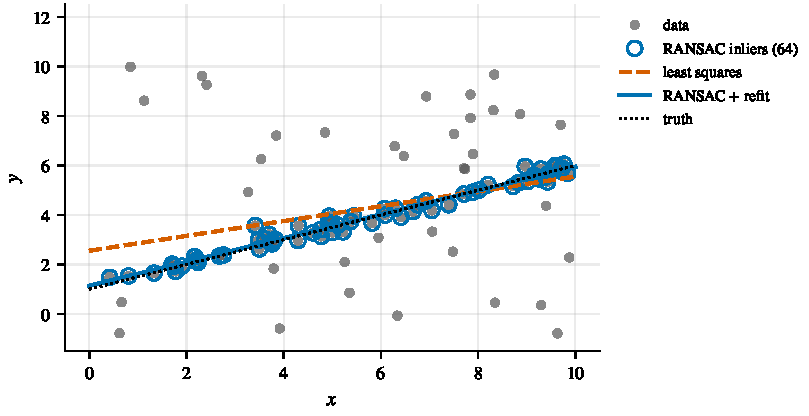
\includegraphics[width=0.86\textwidth]{fig_ransac.pdf}
  \caption{Fitting a line to data with 40\% gross outliers. Least squares is dragged away by the outliers; RANSAC finds the line supported by the most inliers
  (circled) and refits it to them.}
  \label{fig:ransac}
\end{figure}

% ==============================================================================
\section{Degeneracies}

\subsection{Pure rotation}

If the camera only rotates, $t = 0$ and $E = \sx{0}R = 0$: the epipolar constraint is satisfied by every pair of points, inlier or not. Under small translation the problem is
not degenerate but badly conditioned: $t$ is poorly determined, inlier sets fluctuate, and RANSAC may reject good tracks or accept bad ones. Hovering drones rotate in
place often, so this case must be handled (Milestone 9).

Under pure rotation the correspondences satisfy the stronger constraint $\bar x_2 \propto R\bar x_1$ (\cref{sec:homographies}), which does not involve $t$ at all. A robust front end
measures the parallax remaining after rotation compensation, for example the median of $\|\pi(R\bar x_1) - \pi(\bar x_2)\|$ over the tracks:
\begin{itemize}
  \item if it is large, run essential-matrix (or two-point) RANSAC;
  \item if it is tiny, skip epipolar RANSAC and reject only tracks that violate the rotation-only prediction $\bar x_2 \propto R\bar x_1$, with $R$ from the gyroscope.
\end{itemize}
Either way the system keeps tracking: low parallax means the features carry little information about translation, not that they are wrong. The MSCKF update
handles them gracefully, because their nullspace-projected residuals simply contribute little.

\subsection{Other degeneracies}

The eight-point algorithm is degenerate when all points lie on a plane, a common situation (floors, walls), because a homography then explains the data equally well;
the five-point algorithm is not. Very distant points behave like points at infinity and carry only rotational information. Moving objects form a second, consistent
rigid motion that RANSAC can mistake for the dominant one if they fill the image.

% ==============================================================================
\section{Triangulation}
\label{sec:triangulation}

Given observations $z_i$ of a point in cameras with known poses $(R_{wc_i}, p_{wc_i})$, triangulation estimates its world position $p_f$.

\subsection{The midpoint method}

Each observation defines a ray $p_{wc_i} + \lambda_ir_i$ with direction $r_i = R_{wc_i}\bar x_i$. With noise the rays do not intersect. The midpoint method finds the point
closest to all rays in the least-squares sense: the distance of $p$ from ray $i$ is $\|(I - \hat r_i\hat r_i\T)(p - p_{wc_i})\|$ with $\hat r_i$ the unit direction, so
\begin{equation}
  \Big(\sum_i(I - \hat r_i\hat r_i\T)\Big)\,p = \sum_i(I - \hat r_i\hat r_i\T)\,p_{wc_i} .
\end{equation}
It is simple and geometric, but it minimizes 3D distances rather than image errors, which weights distant views wrongly.

\subsection{Linear triangulation}

In camera $i$ the point has coordinates $X_i = R_{wc_i}\T(p_f - p_{wc_i})$, which must be parallel to the bearing $\bar x_i = (z_i, 1)$: $\sx{\bar x_i}X_i = 0$. Substituting,
\begin{equation}
  \sx{\bar x_i}R_{wc_i}\T\, p_f = \sx{\bar x_i}R_{wc_i}\T\, p_{wc_i}, \qquad i = 1,\dots,M .
  \label{eq:dlt}
\end{equation}
Each view contributes three equations of rank two. Stacking all views gives an overdetermined linear system $A p_f = b$ that is solved in the least-squares sense with
QR or SVD. With two views and noise-free data the solution is exact. This is the linear initialization of AGENTS.md F5. It minimizes an algebraic error, not the
reprojection error, so it is refined next.

\subsection{Nonlinear refinement with inverse depth}

The maximum-likelihood estimate minimizes the reprojection error (\cref{ch:nlls})
\begin{equation}
  \min_{p_f}\ \sum_{i=1}^M \big\| z_i - \pi(X_i(p_f)) \big\|^2 .
\end{equation}
The MSCKF~\cite{mourikis2007msckf} parameterizes the point in an \emph{anchor} camera $A$ (for example the first observation) by inverse depth~\cite{civera2008inverse}:
\begin{equation}
  X_A = \frac1\rho\begin{bmatrix} \alpha \\ \beta \\ 1 \end{bmatrix}, \qquad
  X_i = R_{iA}X_A + p_{iA}
  \quad\Longrightarrow\quad
  h_i := \rho X_i = R_{iA}\begin{bmatrix}\alpha\\ \beta\\ 1\end{bmatrix} + \rho\,p_{iA}, \quad z_i = \pi(h_i),
\end{equation}
where $(R_{iA}, p_{iA})$ is the transformation from the anchor camera to camera $i$, computed from the clone poses, and $\pi(h_i) = \pi(X_i)$ because projection ignores scale.
The parameters $(\alpha, \beta)$ are the normalized coordinates in the anchor view and $\rho = 1/Z_A$ is the inverse depth. This parameterization behaves well for distant points
($\rho\to0$ is a regular point), and the measurement function is nearly linear in $(\alpha, \beta, \rho)$. Its Jacobian follows from the chain rule:
\begin{equation}
  \frac{\partial z_i}{\partial(\alpha, \beta, \rho)} = \frac{\partial\pi}{\partial h}\Big|_{h_i}\,
  \begin{bmatrix} r_1 & r_2 & p_{iA} \end{bmatrix},
\end{equation}
where $r_1, r_2$ are the first two columns of $R_{iA}$ and $\partial\pi/\partial h$ is \cref{prop:proj-jacobian}. Gauss--Newton (\cref{alg:gauss-newton}) iterates
$\delta y = -(J\T J)\inv J\T e$ with the stacked Jacobian $J$ and residual $e$, usually converging in a few iterations from the linear initialization. Levenberg--Marquardt
damping adds robustness.

\subsection{How accurate is triangulation?}

For two views separated by a baseline $b$ perpendicular to the viewing direction, the depth is $Z = b/d$ with $d$ the disparity in normalized coordinates. With
independent noise $\sigma_{uv}$ in each view, $\sigma_d = \sqrt2\sigma_{uv}$, and since $\partial Z/\partial d = -b/d^2 = -Z^2/b$, to first order
\begin{equation}
  \sigma_Z \approx \frac{Z^2}{b}\sqrt2\,\sigma_{uv} .
  \label{eq:depth-sigma}
\end{equation}
Depth error grows quadratically with depth and inversely with baseline. Equivalently, the relative depth error is inversely proportional to the parallax angle $\approx b/Z$.

\begin{figure}[t]
  \centering
  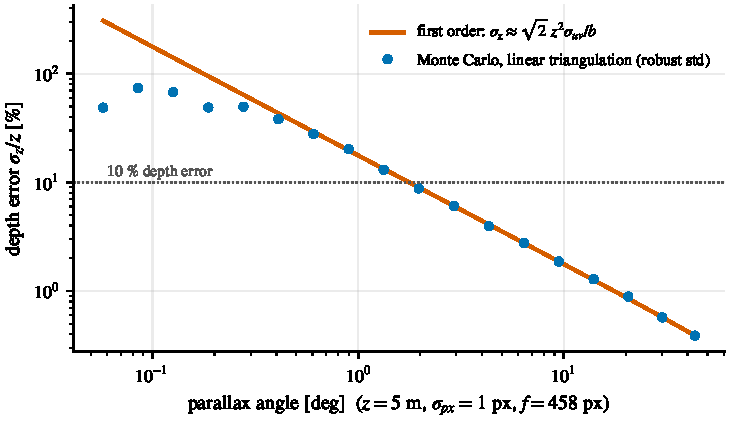
\includegraphics[width=0.86\textwidth]{fig_triangulation.pdf}
  \caption{Relative depth error of two-view triangulation at $Z = 5$~m with 1-pixel noise, versus parallax angle. Down to about $1^\circ$ the first-order formula \eqref{eq:depth-sigma}
  describes the spread accurately. Below that the error distribution becomes heavy-tailed (depths can even become negative), and the estimate is unusable.}
  \label{fig:triangulation}
\end{figure}

\Cref{fig:triangulation} shows that 10\% depth accuracy needs about $2^\circ$ of parallax, a baseline of 17~cm at 5~m. Down to about $1^\circ$ \eqref{eq:depth-sigma} still
describes the bulk of the estimates; below that, outliers take over. At $0.5^\circ$, 4\% of the estimates are off by more than five standard deviations, and at
$0.25^\circ$, 8\% of the depths come out negative. A triangulation module must therefore check its own result before handing it to the filter:
\begin{itemize}
  \item positive depth in every view (cheirality);
  \item sufficient parallax (or baseline relative to depth), or equivalently a well-conditioned Gauss--Newton Hessian;
  \item small reprojection error in every view after refinement;
  \item a plausible depth range.
\end{itemize}
Features that fail are discarded, not fed to the update (AGENTS.md F5, Milestone 10b).

% ==============================================================================
\section{Bundle adjustment}
\label{sec:bundle-adjustment}

\termi{Bundle adjustment}{bundle adjustment} estimates all camera poses and all 3D points at once by minimizing the total reprojection error,
\begin{equation}
  \min_{\{T_i\},\{p_j\}}\ \sum_{(i,j)\text{ observed}}\big\|z_{ij} - \pi\big(T_i\inv p_j\big)\big\|^2_{R\inv},
\end{equation}
with Gauss--Newton or Levenberg--Marquardt on the manifold of poses (\cref{ch:nlls}). It is the gold standard of geometric vision. Two of its properties illuminate
VIO.
\begin{itemize}
  \item \emph{Structure.} Each residual involves one camera and one point, so the normal equations have the block structure of \cref{sec:schur-ba}: eliminating the
        points with the Schur complement leaves a small \emph{reduced camera system} (\cref{fig:ba-sparsity}).
  \item \emph{Gauge freedom.} Moving and rotating everything together, or (for a monocular camera) scaling everything, leaves all reprojection errors unchanged: the
        problem has seven unobservable directions, and $J\T WJ$ is singular along them. Solvers fix the gauge by holding the first camera fixed and the scale constant, or
        by adding a weak prior. With an IMU, scale and two rotation directions (roll and pitch) become observable, and the gauge shrinks to the four directions of
        \cref{ch:observability}.
\end{itemize}
The MSCKF can be understood as a fast, filtered approximation of bundle adjustment over a sliding window: it eliminates each point exactly as the Schur complement
does (\cref{ch:msckfupdate}), takes a single Gauss--Newton step, and summarizes the past by the filter's Gaussian prior instead of relinearizing it.

\paragraph{Pose from known points.} Finally, when the 3D points are known (a map), a single image determines the camera pose: the
\emph{perspective-$n$-point} (PnP) problem, solved minimally from three points and refined by Gauss--Newton. It is the core of relocalization against a map, a
capability that odometry lacks.

\begin{takeaways}
\begin{itemize}
  \item Rigid correspondences satisfy $\bar x_2\T\sx{t}R\bar x_1 = 0$; $E$ has 5 DOF, singular values $(\|t\|, \|t\|, 0)$, and an unobservable scale.
  \item The eight-point algorithm is linear (normalize pixel coordinates first); $E$ decomposes into four motions, one of which passes the cheirality test.
  \item With the rotation from the gyroscope, two correspondences determine the translation direction.
  \item Planes and pure rotations relate views by homographies; under pure rotation $E$ vanishes and the rotation-only constraint takes over.
  \item RANSAC iterations grow as $w^{-s}$: prefer minimal solvers. Thresholds in normalized units are $\tau_{px}/f$.
  \item Triangulate linearly, refine by Gauss--Newton with inverse depth, and reject low-parallax or negative-depth points; depth error grows as $Z^2/b$.
  \item Bundle adjustment is the batch problem; the MSCKF approximates it with exact landmark elimination and a single Gauss--Newton step.
\end{itemize}
\end{takeaways}

\begin{exercises}
  \item Verify \cref{thm:epipolar} numerically for random points and a random relative pose, then show that adding an outlier breaks it.
  \item Prove \cref{prop:essential} and show that $e_2 \propto t$ is the left null vector of $E$.
  \item Implement the eight-point algorithm with and without Hartley normalization on pixel coordinates, and compare the errors.
  \item Implement the decomposition of \cref{prop:e-decomposition} and the cheirality test, and verify on synthetic data that the correct solution is selected.
  \item Implement the two-point method with known rotation inside RANSAC on synthetic data with 30\% outliers. Compare the number of iterations needed with the five-point
        method.
  \item Generate a pure-rotation sequence, observe what \code{cv::findEssentialMat} returns, and implement the parallax test.
  \item Show that \eqref{eq:dlt} has rank two per view and that two views with non-parallel rays give a unique solution.
  \item Derive \eqref{eq:depth-sigma}, reproduce \cref{fig:triangulation}, and repeat with three views over the same baseline.
  \item Count the gauge freedoms of monocular bundle adjustment and of visual-inertial bundle adjustment, and explain the difference.
\end{exercises}
% Solutions to the exercises of Chapter 23.
\begin{solutions}
  \item With 20 random points at 3--8~m and a random relative pose, $|\bar x_2\T E\bar x_1| \le 3\times10^{-17}$: rounding error. Moving one observation in the second image
        by 27~px gives an algebraic residual of $8\times10^{-3}$ and a Sampson distance $\sqrt{d_S}$ of $5.4$~px. Only the component of the error perpendicular to the
        epipolar line is visible (7.7~px of the 27~px here), and the Sampson distance spreads it over both images ($7.7/\sqrt2 = 5.4$). A two-view check cannot
        detect an error \emph{along} the epipolar line at all; a third view, or the filter's own gating, must catch those.

  \item Since $RR\T = I$ and $\sx{t}\T = -\sx{t}$, $EE\T = -\sx{t}^2 = \|t\|^2I - tt\T$ (\eqref{eq:skew-sq}). Every vector orthogonal to $t$ is an eigenvector with eigenvalue
        $\|t\|^2$, and $t$ itself has eigenvalue 0, so the singular values of $E$ are $(\|t\|, \|t\|, 0)$ and its rank is two. Degrees of freedom: $R$ has three and $t$ three,
        but the constraint $\bar x_2\T E\bar x_1 = 0$ is homogeneous, so $E$ and $\lambda E$ (i.e.\ $t$ and $\lambda t$) are indistinguishable: $3 + 2 = 5$. Scaling the scene and
        the baseline together leaves every bearing unchanged, so the scale of $t$ cannot be recovered from images. For the epipoles,
        \[
          t\T E = t\T\sx{t}R = -(\sx{t}t)\T R = -(t\times t)\T R = 0, \qquad E(R\T t) = \sx{t}t = 0 .
        \]
        The left null vector is $t$, the coordinates of the first camera center in the second frame ($X_1 = 0 \Rightarrow X_2 = t$), so $e_2 \propto t$ is its image. Likewise
        $e_1 \propto R\T t$ is the image of the second center ($X_2 = 0 \Rightarrow X_1 = -R\T t$).

  \item With 60 points, 0.5~px noise and 200 random scenes, recovering $(R, t)$ from $E = K\T FK$:
        \begin{center}\small
        \begin{tabular}{@{}l c c c@{}}
        \toprule
        & $\sigma_1/\sigma_8$ of $A$ & rotation error & direction of $t$ \\
        & & median / 90\% & median / 90\% \\
        \midrule
        raw pixels & $1.5\times10^5$ & $0.33^\circ$ / $1.6^\circ$ & $2.5^\circ$ / $11^\circ$ \\
        Hartley-normalized & 66 & $0.16^\circ$ / $0.34^\circ$ & $1.1^\circ$ / $2.4^\circ$ \\
        \bottomrule
        \end{tabular}
        \end{center}
        In pixels, the columns of $A$ range from $1$ to $10^5$, so the smallest singular vector is dominated by rounding and by the noise in the large entries.
        Normalization makes all columns comparable. It halves the typical error and removes the bad cases, which matter most inside RANSAC.

  \item Take the SVD of $E$, flip the sign of $U$ or $V$ if its determinant is $-1$ (allowed, since $E$ is defined up to sign), and form the four candidates. For each,
        triangulate every correspondence (two depths from $\lambda_2\bar x_2 = \lambda_1R\bar x_1 + t$ by least squares) and count the points with both depths positive. In 500 random
        scenes, the true solution won every time, with all points in front of both cameras. For each wrong candidate, \emph{all} points failed: in a typical scene one
        candidate put them in front of the first camera but behind the second, and the other two put them behind the first. With noisy data, use the count, not
        a requirement that every point pass.

  \item With $R$ known, each correspondence gives $c_i = R\bar x_1^{(i)}\times\bar x_2^{(i)}$, the hypothesis is $t \propto c_i\times c_j$, and inliers have $\sqrt{d_S}$ below the threshold (2~px).
        For 100 correspondences with 1-pixel noise and 30\% outliers, adaptive RANSAC stopped after 9.8 iterations on average ($\lceil\log0.01/\log(1 - 0.7^2)\rceil = 7$
        at the true ratio; the observed ratio is slightly lower because the threshold rejects some inliers). After refitting $t$ to all inliers (the unit $t$
        minimizing $\sum(t\T c_i)^2$), the median direction error was $0.6^\circ$; 4.6\% of the inliers were rejected (the expected rate of a $2\sigma$ threshold) and 1.3\% of the
        outliers accepted (those lying near their epipolar line by chance). The five-point method needs $\lceil\log0.01/\log(1 - 0.7^5)\rceil = 26$ iterations at the same confidence,
        each solving a degree-10 polynomial and scoring up to ten candidates, against one cross product. The price of the two-point method is its dependence
        on the gyroscope: a rotation error $\delta$ shifts predicted points by about $f\delta$ pixels, so the threshold must cover the gyro error accumulated between
        frames.

  \item With $t = 0$, every correspondence satisfies $\bar x_2 \propto R\bar x_1$, so $\bar x_2\T\sx{t}R\bar x_1 = \bar x_2\T(t\times R\bar x_1) = 0$ for \emph{every} $t$. The data fit the
        whole family $E = \sx{t}R$, and the eight-point matrix $A$ has three singular values at the noise level instead of one. In simulation, a randomly chosen
        $t$ combined with the true $R$ fits 68--70\% of the tracks to within 1~px, exactly the fraction the true model fits with 1-pixel noise. Whatever
        \code{cv::findEssentialMat} returns therefore has an arbitrary translation direction that changes from run to run, and its inlier set is no test of the
        tracks, since the free $t$ can turn epipolar lines through outliers. The parallax test: the median of $\|\pi(R\bar x_1) - \pi(\bar x_2)\|$ over the tracks was
        $1.6$~px under pure rotation (noise only) and $8.8$~px for a 10~cm sideways motion with points at 3--8~m. A threshold of a few pixels separates the two
        regimes. Below it, check tracks only against $\bar x_2 \propto R\bar x_1$.

  \item The matrix $\sx{\bar x_i}$ has rank two (its nullspace is $\bar x_i$), and multiplying by the invertible $R_{wc_i}\T$ keeps the rank, so each view contributes three
        equations of rank two. For two views, $p$ is in the nullspace of the stacked matrix if and only if $R_{wc_i}\T p \parallel \bar x_i$ for both views, i.e.\ $p$ is parallel to both ray
        directions $r_i = R_{wc_i}\bar x_i$. If the rays are not parallel, only $p = 0$ qualifies: the $6\times3$ matrix has full column rank, and the least-squares solution
        is unique. Parallel rays (zero parallax) leave a one-dimensional nullspace, the position along the ray.

  \item With the baseline perpendicular to the viewing direction, $Z = b/d$ with disparity $d = x_1 - x_2$. The two noises are independent, so $\sigma_d = \sqrt2\sigma_{uv}$, and to first
        order $\sigma_Z = |\partial Z/\partial d|\,\sigma_d = (b/d^2)\sqrt2\sigma_{uv} = (Z^2/b)\sqrt2\sigma_{uv}$. A Monte Carlo at $Z = 5$~m with 1-pixel noise reproduces the figure: relative errors
        of $17.7\%$, $8.8\%$, $3.5\%$, $1.8\%$ at parallax angles of $1^\circ$, $2^\circ$, $5^\circ$, $10^\circ$, matching the formula. For three views at $0$, $b/2$ and $b$, write the
        observations as $x_i = X/Z - s_i/Z + n_i$, with $s_i$ the camera positions along the baseline. The inverse depth $1/Z$ is the \emph{slope} of a straight-line fit of $x_i$
        against $s_i$, with variance $\sigma_{uv}^2/\sum_i(s_i - \bar s)^2$. A view at the mean position $\bar s$ adds nothing to this sum: three views give the same depth accuracy as
        two (simulation: within 2\%), and five equally spaced views improve it by only 11\%. Depth accuracy is bought with baseline; intermediate views
        add redundancy, which is what outlier detection and the MSCKF's nullspace projection need.

  \item Monocular bundle adjustment has seven gauge freedoms: a global translation (3), a global rotation (3) and a global scale (1) leave all reprojection errors
        unchanged. Visual--inertial bundle adjustment has four: translation (3) and rotation about the gravity direction (1). The accelerometer measures
        specific force in the body frame, and the residuals compare it with $R_{wb}\T(a_w - g_w)$ for the fixed $g_w$. A global rotation about a horizontal axis would tilt the
        trajectory relative to gravity and change these residuals, so roll and pitch are observable. A rotation about the vertical leaves $g_w$ invariant and
        changes nothing. Scale becomes observable because the IMU measures metric accelerations, which a scaled trajectory would contradict, provided
        the motion actually accelerates (at constant velocity, scale is unobservable again). Consequently, fix the gauge of a visual--inertial problem with
        the first position and yaw only: fixing roll and pitch as well would inject false information.
\end{solutions}

